\section{Data structure}

\subsection{Normality test}
\begin{center}
	\begin{figure}[H]
		\subfloat[Raw data]{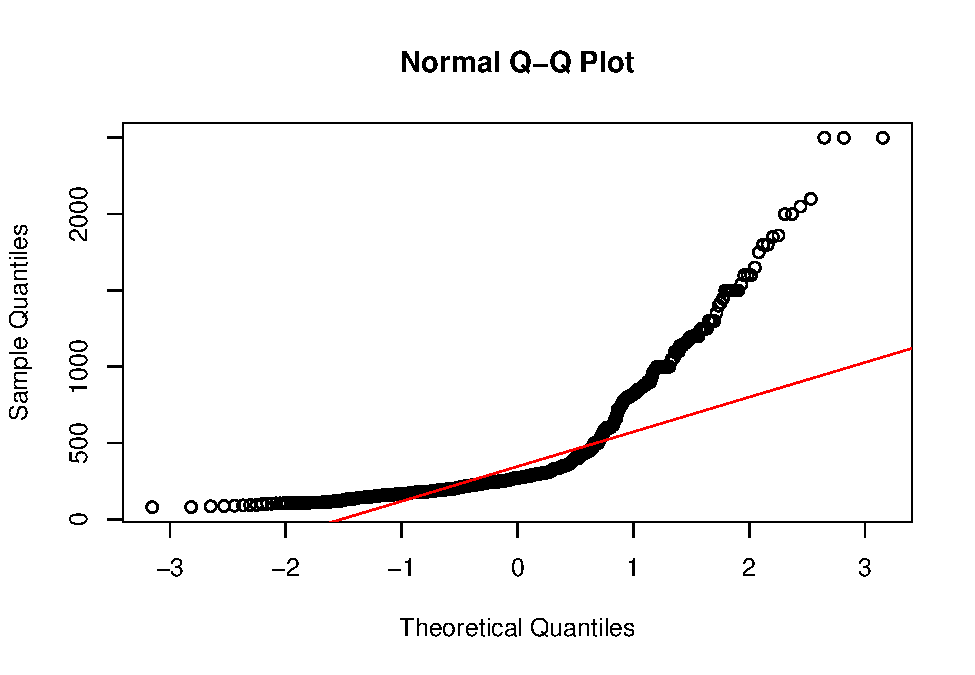
\includegraphics[scale=0.45]{MA_JJ_files/figure-latex/normalDistribution-1.pdf}}
		\subfloat[Logtransformed data]{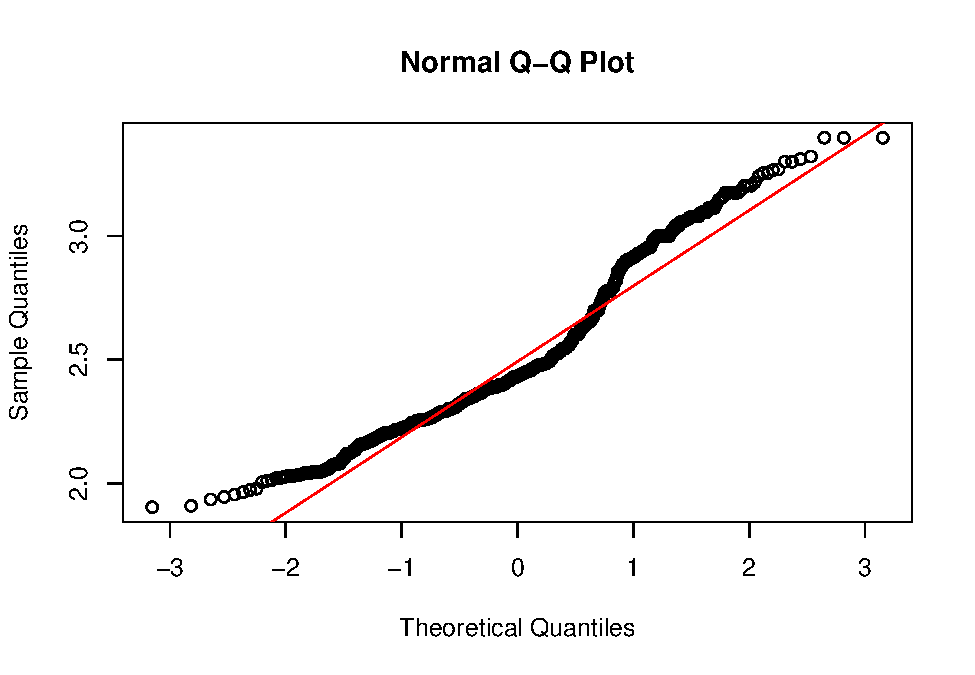
\includegraphics[scale=0.45]{MA_JJ_files/figure-latex/normalDistribution-2.pdf}}	
		\caption[Testing normal distribution]{Visual test for normal distribution. In case of normally distributed data, the black circles should follow the red line, which is not the case for either raw data (a) nor logtransformed data (b). Therefore, data is assumed to not be normally distributed and nonparametric test are used for all statistical analyses.}
		\label{fig:NormDis}
	\end{figure}
\end{center}


\begin{center}
	\begin{figure}[H]
		\subfloat[Comparison of carapace length of modern and fossil continental/insular \T ]{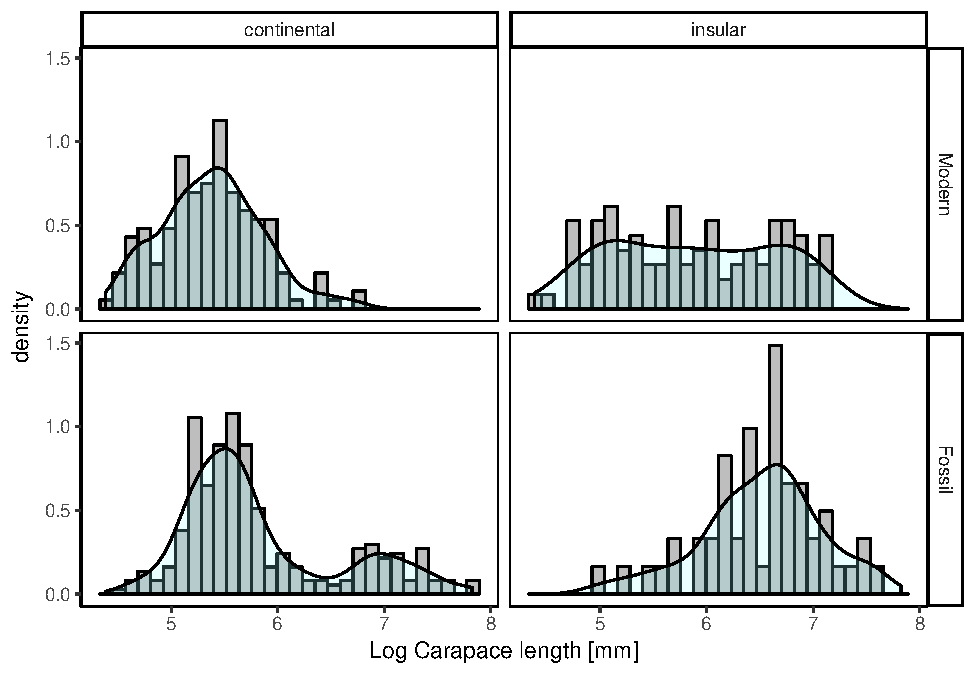
\includegraphics[scale=0.45]{MA_JJ_files/figure-latex/HistFMCI-1.pdf}}
		\subfloat[Comparison of carapace length among continents]{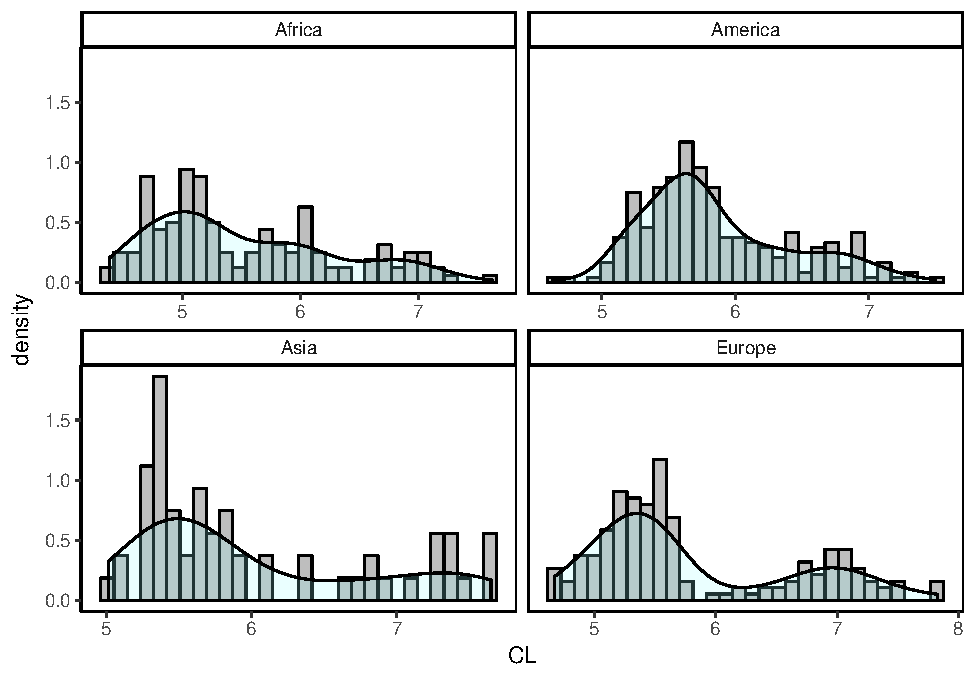
\includegraphics[scale=0.45]{MA_JJ_files/figure-latex/HistCon-1.pdf}}	
		\caption[Comparison of carapace lengths in subgroups]{Body size distribution of subgroups. (a) Comparison of body size in modern continental and modern insular as well as fossil continental and fossil insular testudinids. Fossil continental testudinids reflect the bimodal distribution of the complete dataset, but large testudinids are missing in modern continental testudinids. Fossil insular testudinids are strongly left-skewed, whereas modern insular testudinids show a rather flat distribution. (b) Comparison of carapace length among continents. All continents roughly reflect the bimodal distribution of the complete dataset.}
		\label{fig:HistRest}
	\end{figure}
\end{center}